\documentclass[10pt,a4paper]{ULBreport}
\usepackage[utf8]{inputenc}
\sceau{pic/official_logos/sceauULB.png}
\graphicspath{ {./pic/} }
\usepackage{multirow}
\usepackage{listings}
\usepackage{color} 
\usepackage{setspace} 
\usepackage{amsmath}
\usepackage{mathrsfs}
\usepackage{bm}
\usepackage[mathscr]{eucal}
\usepackage{hyperref}
\usepackage{pdfpages}
\usepackage{biblatex}
\usepackage{floatrow}
\usepackage{subcaption} 
\usepackage{siunitx}
\usepackage[many]{tcolorbox}
\usepackage{multirow}
\usepackage{listings}
\usepackage[dvipsnames]{xcolor}
\usepackage{fancyvrb}
\usepackage{graphicx}

\usepackage{xstring}
\usepackage{etoolbox}

% Colors



\begin{document} 


	\titleULB{
	title={V2V communication project},
    studies={M1-IRELE},
    course ={ELEC-H415 Communication Channels},
    author={\textit{Author :} \\ Colot Emmeran },
    date={\textbf{Academic year :} \\ 2024 - 2025},
    teacher={\textit{Professor : } \\ De Doncker Philippe},
    logo={pic/official_logos/logos.jpg},
    manyAuthor
	}

%\listoftables % ToC for tables

%\listoffigures % ToC for figures

\chapter{Introduction}

\begin{center}
    
    \Huge TODO\\
    \vspace{0.5cm}
    \large Might want to check all 3d plots names\\
    Write an introduction\\
    Resize figures to fill pages
    \normalsize
    
\end{center}
\chapter{Theoretical answers}

\section{$\lambda/2$ antennas}

\begin{figure}[H]
    \centering
    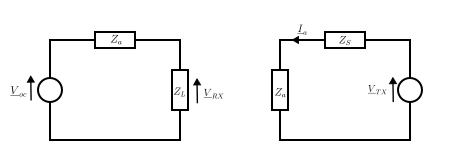
\includegraphics[width=1\textwidth]{circuit.png}
    \caption{Equivalent electric circuit of the RX antenna (left) and the TX antenna (right)}
    \label{fig:equivalent_electrical_circuit}
\end{figure}

Fig \ref{fig:equivalent_electrical_circuit} shows the equivalent electrical circuit at RX and TX where $\underline{V}_{oc}$ is the induced voltage, $\underline{V}_{\text{RX}}$ the voltage at the output of the RX antenna, $\underline{V}_{\text{TX}}$ the one at the input of the TX antenna and $\underline{I}_{a}$ the current entering the TX antenna.\\

As both antennas are vertical $\lambda/2$ dipoles, their equivalent heights can be analytically computed:

\begin{align*}
    \vec{h}_e (\theta, \phi) = \frac{\lambda}{\pi} \frac{\cos\left(\frac{1}{2}\cos \theta\right)}{\sin ^2 \theta}\vec{1_z}\\
    \vec{h}_{e\perp} (\theta, \phi) = -\frac{\lambda}{\pi} \frac{\cos\left(\frac{\pi}{2}\cos \theta\right)}{\sin \theta}\vec{1_\theta}
\end{align*}

Where $\theta$ and $\phi$ are respectively the polar and the azimuthal angles. This means that the horizontal plane (in which the rays in the simulation propagating) corresponds to $\theta = \pi/2$. The transverse equivalent height is then reduced to the following, where it does not depend on the azimuthal angle $\phi$:

\begin{align*}
    \vec{h}_{e\perp} (\phi) = -\frac{\lambda}{\pi} \vec{1_{\theta}}\\
\end{align*}

The transverse part of the equivalent height gives rise to an expression for the emitted electric field.

\begin{align*}
    \underline{\vec{E}}(\vec{r}) &= -j\omega \underline{I}_a \frac{\mu_0}{4\pi}\frac{e^{-j\beta r}}{r}\vec{h}_{e\perp}(\theta, \phi) \\
    &= j\omega \underline{I}_a \frac{\mu_0\lambda}{4\pi^2}\frac{e^{-j\beta r}}{r} \vec{1_{\theta}} \\
    &= j \frac{\underline{I}_a \mu_0 c}{2\pi} \frac{e^{-j\beta r}}{r} \vec{1_{\theta}}\\
    &= j \frac{\underline{I}_a Z_0}{2\pi} \frac{e^{-j\beta r}}{r} \vec{1_{\theta}}
\end{align*}

To make the transmission parameters appear in the electric field expression, $\beta$ and $\underline{I}_a$ must be replaced with the formulas given below.

\begin{equation*}
    \beta = \frac{2\pi f_c}{c}
\end{equation*}
\begin{equation*}
    \underline{V}_{\text{TX}} = (Z_a + Z_S) \underline{I}_a
\end{equation*}

Wich yields

\begin{equation*}
    \underline{\vec{E}}(\vec{r}) = j \frac{\underline{V}_{\text{TX}}}{2\pi}\frac{Z_0}{Z_a + Z_S} \frac{e^{-\frac{j2\pi f_c r}{c}}}{r} \vec{1_{\theta}}
\end{equation*}

The last step is to replace the travel distance $r$ with $c \tau$ as the wave is propagating at the speed of light in free space. The electric field thus becomes:

\begin{equation*}
    \underline{\vec{E}}(\vec{r}) = j \frac{\underline{V}_{\text{TX}}}{2\pi}\frac{Z_0}{Z_a + Z_S} \frac{e^{-j2\pi f_c \tau}}{c\tau} \vec{1_{\theta}}
\end{equation*}

The voltage at the output of the antenna $\underline{V}_{\text{RX}}$ can be deduced from the equivalent electric circuit \ref{fig:equivalent_electrical_circuit} as it is a simple voltage divider. Assuming matching impedances between the antenna and the load, we have:

\begin{align*}
    \underline{V}_{\text{RX}} = \frac{Z_L}{Z_a + Z_L} \underline{V}_{oc} = \frac{1}{2} \underline{V}_{oc}\\
    \underline{V}_{oc} = -\left . \vec{h}_{e\perp}(\theta, \phi)\right\vert_{\theta = \pi/2} \cdot \underline{\vec{E}}_i
\end{align*}

Where $\underline{\vec{E}}_i = - \underline{\vec{E}}$ due to the change of coordinates origin. It is here assumed that there was no reflexion, refraction or transmission through another material. This allows to find the votages at the receiver side as a function of the voltage at the transmitter side.

\begin{align*}
    \underline{V}_{oc} &= \frac{\lambda}{\pi} \cdot \underline{E}_i\\
    &= -j\frac{\lambda\underline{V}_{\text{TX}}}{2\pi^2}\frac{Z_0}{Z_a + Z_S}\frac{e^{-j 2\pi f_c \tau}}{c\tau}\\
    \underline{V}_{\text{RX}} &= -j\frac{\lambda}{4\pi^2}\frac{Z_0}{Z_a + Z_S}\frac{e^{-j 2\pi f_c \tau}}{c\tau} \underline{V}_{\text{TX}}
\end{align*}

For later use, the time of flight $\tau$ is replaced by the traveled distance $d$, which is more convenient for the simulation. $Z_0$, $Z_a$, and $Z_S$ can also be replaced by $120\pi$, $\frac{720\pi}{32}$, and $\frac{720\pi}{32}$, respectively (assuming once again that the impedances are matched).\\

\begin{align}
    \underline{V}_{\text{RX}} &= -j\frac{2 \lambda }{3\pi^2}\frac{e^{-j\frac{2\pi f_c d}{c}}}{d}\underline{V}_{\text{TX}}
    \label{eq:voltage_RX}
\end{align}

\section{LOS channel}
\label{sec:LOS_channel}

Assuming the communication takes place via a LOS ray only, the channel impulse response $h(\tau)$ is defined as follows:

\begin{align*}
    h(\tau) = \frac{\alpha_1 e^{-j\frac{2\pi f_cd_1}{c}}}{d_1} \delta\left(\tau - \tau_1\right)
\end{align*}

Where $d_1$ is the distance of propagation and $\tau_1$ he propagation delay of the direct ray. $\alpha_1$ (which might be complex) takes into account a phase change or attenuation due for example to reflections whereas the imaginary exponential next to it corresponds to the phase change due to the propagation delay. In the case of LOS transmission $\alpha_1$ is equal to 1.\\
The transfer function $H(f)$ of the channel is found by taking the Fourier transform of $h(\tau)$

\begin{align*}
    H(f) &= \int_{-\infty}^{\infty} h(\tau) e^{-j2\pi f \tau} d\tau\\
    &= \frac{e^{-j\frac{2\pi f_c d_1}{c}}}{d_1}e^{-j2\pi f \frac{d_1}{c}}\\
    &= \frac{e^{-j \frac{2\pi (f+f_c)d_1}{c}}}{d_1}\\
\end{align*}

% FALSE ???
% As we consider a single ray, the narrowband model of the channel $h_{\text{NB}}$ (representing the case where the receiver perceives the sum of all propagation path) is simply found by removing the Dirac pulse from $h(\tau)$

% \begin{align*}
%     h_{\text{NB}} = \frac{e^{-j \frac{2\pi f_cd_1}{c}}}{d_1}
% \end{align*}

The narrowband impulse response of the channel $h_{\text{NB}}(\tau)$ is, in the case of a single ray, simply equal to $h(\tau$) and the signal received at the output of the channel $y(t)$ is given by:

\begin{equation*}
    y(t) = h_{\text{NB}}(t) x(t)
\end{equation*}
\begin{equation*}
    \text{where} \qquad h_{\text{NB}}(t) = h(t) = \frac{e^{-j \frac{2\pi f_cd_1}{c}}}{d_1} \delta(t - \tau_1)
\end{equation*}

Where $x(t)$ is the transmitted signal. \\
The ratio between the received power $P_{\text{RX}}$ and the transmitted power $P_{\text{TX}}$ is found with:

\begin{align}
    \frac{P_{\text{received}}}{P_{\text{transmitted}}} &= \frac{\left| h(\tau) \right|^2}{2} \nonumber\\
    &= \frac{1}{d_1^2}
    \label{eq:power_approx}
\end{align}

This result can be compared with the Friis formula, given by:

\begin{align}
    P_{\text{RX}}(d) = P_{\text{TX}} G_{\text{TX}}(\theta_{\text{TX}}, \phi_{\text{TX}})G_{\text{RX}}(\theta_{\text{RX}}, \phi_{\text{RX}})\left(\frac{\lambda}{4\pi d}\right)^2
    \label{eq:friis_formula}
\end{align}

The reason for the big difference between the two formulas can be easily explained: in eq \ref{eq:power_approx}, $P_{\text{transmitted}}$ and $P_{\text{received}}$ are the powers of the waves, not the one of the signal before/after passing through the antennas. To correct it, they are replaced by the Poynting vectors $\bm{\vec{\mathscr{S}}}_{\text{TX}}$ and $\bm{\vec{\mathscr{S}}}_{\text{RX}}$:

\begin{align}
    \frac{\left|\bm{\vec{\mathscr{S}}}_{\text{RX}}\right|}{\left|\bm{\vec{\mathscr{S}}}_{\text{TX}}\right|} = \frac{1}{d_1^2}
    \label{eq:poynting}
\end{align}

To compare the received and the injected power, the Poynting vectors should be replaced by

\begin{align*}
    \left|\bm{\vec{\mathscr{S}}}_{\text{TX}}\right| = G_{\text{TX}} P_{\text{TX}}\\
    \left|\bm{\vec{\mathscr{S}}}_{\text{RX}}\right| A_{eRX} = P_{\text{RX}}\\
    \text{where} \quad \quad A_{eRX} = G_{\text{RX}}\left(\frac{\lambda}{4\pi}\right)^2
\end{align*}

When placed back in eq \ref{eq:poynting}, the expression matches the Friis formula (eq \ref{eq:friis_formula}). \\
To further simplify and as the antennas are considered to be lossless dipoles, equation \ref{eq:power_friis_simplified} replaces their gain by $\frac{16}{3\pi}$, the theoretical gain of such antennas.

\begin{align}
    \frac{P_{\text{RX}}}{P_{\text{TX}}} &= G_{\text{TX}} G_{\text{RX}} \left(\frac{\lambda}{4\pi d_1}\right)^2\\
    \label{eq:power_friis_simplified}
    &= \frac{16}{9\pi^2} \left(\frac{\lambda}{\pi d_1}\right)^2
\end{align}

Two deductions can be made of this result: 
\begin{itemize}
    \item The power loss on the channel depends on the square of the distance between the emitter and the receiver. It implies that doubling the range of an antenna would need a multiplication of the transmitting power by a factor 4.
    \item A more surprising result is the wavelength squared appearing at the numerator. It shows that there is always a compromise between data rate and power consumption as a larger wavelength will indeed be less attenuated but the maximal data rate will then be lowered in order for the channel to still be considered as narrowband.
\end{itemize}

\chapter{Simulation results}
\section{Raytracing}

After having implemented a raytracing algorithm, the simulation is able to compute every path from the transmitter to the receiver. Figure \ref{fig:raytracingDemo} shows the result of the simulation for cars spaced by 100m on a 20m wide road surrounded by buildings. For a better understanding, the angles are computed between the buildings and the rays. This is only done on this graph as the angles used to compute the reflection coefficients $\Gamma_{\perp}$ are the ones between the normal to the obstacle and the ray.

\begin{figure}[H]
    \centering
    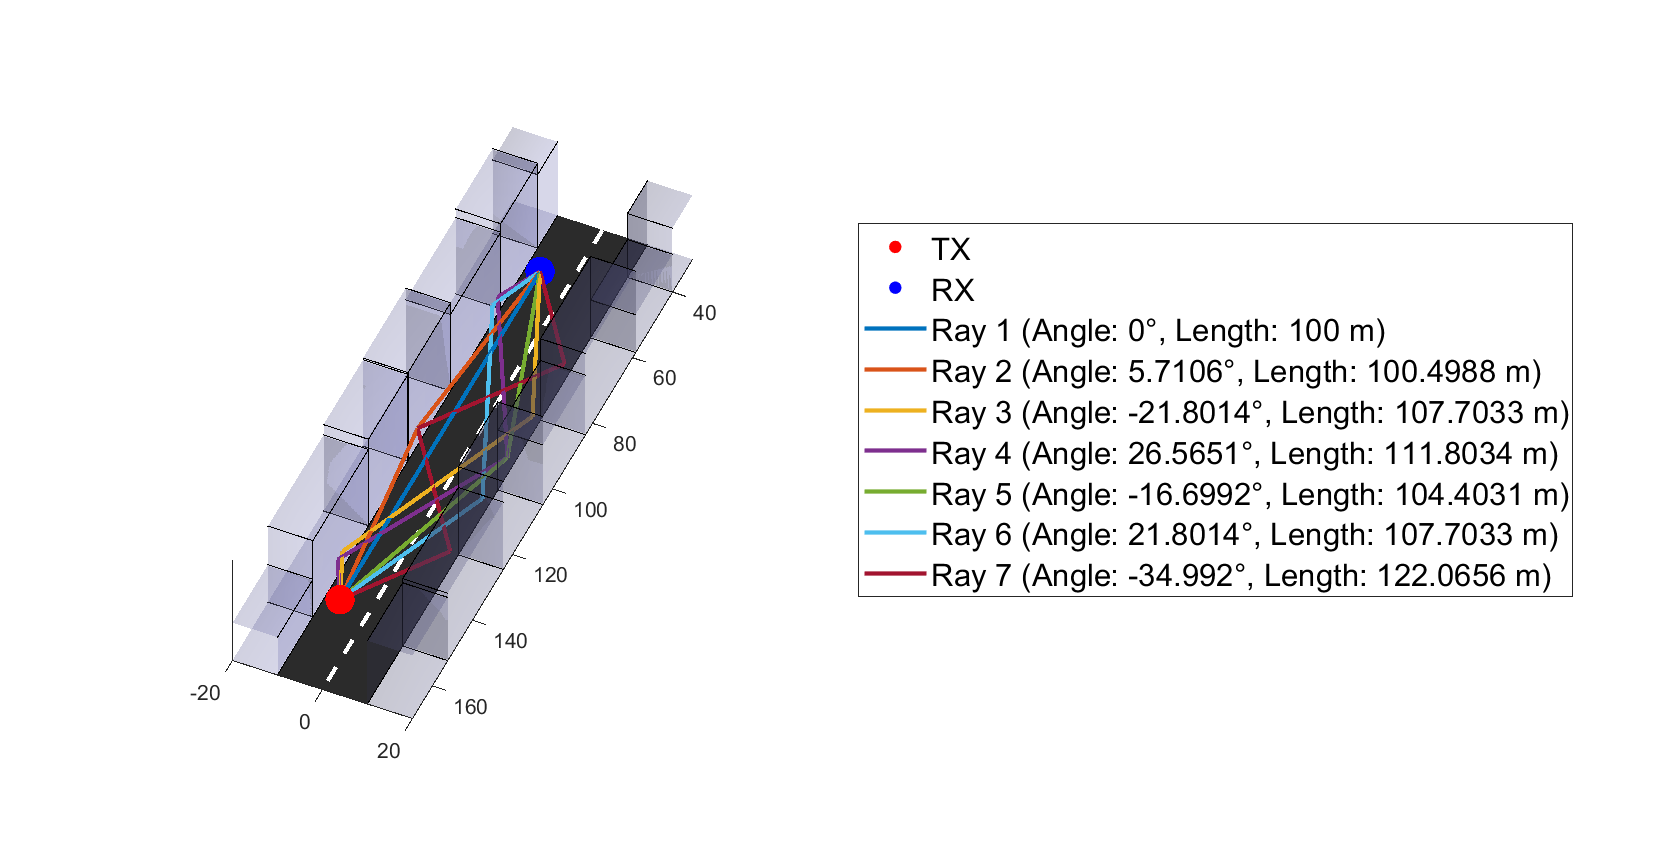
\includegraphics[width=1\textwidth]{3_1.eps}
    \caption{Raytracing simulation of a road surrounded by buildings}
    \label{fig:raytracingDemo}
\end{figure}

The received voltage has been computed on the same setup using equation \ref{eq:voltage_RX} to which the reflection coefficients $\Gamma_{\perp}$ have been added. 

\begin{align*}
    \Gamma_{\perp} = \frac{\cos \theta_i - \sqrt{\epsilon_r-\sin^2\theta_i}}{\cos \theta_i + \sqrt{\epsilon_r-\sin^2\theta_i}}
\end{align*}

The voltage carried by each ray is shown in figure \ref{fig:voltageDemo} using a colormap and the exact values are given in table \ref{tab:ray_properties}. The total received voltage is computing by summing the voltages of each ray and taking the phase into account. This gave the following result:

\begin{align*}
    \text{Total voltage} = 145.6 \mu V \angle -48.8^\circ
\end{align*}

\begin{table}[H]
    \centering
    \begin{tabular}{|c|c|c|c|c|}
        \hline
        Ray Index & Ray physical angle (°) & Ray length (m) & Carried voltage ($\mu V$) & Phase (°) \\ \hline
        1 & 180.0 & 100.0 & 129.1 & 30.0\\ \hline
        2 & 174.3 & 100.5 & 114.6 & -81.2\\ \hline
        3 & -163.3 & 104.4 & 88.9 & -3.7\\ \hline
        4 & -158.2 & 107.7 & 51.2 & -149.3\\ \hline
        5 & 158.2 & 107.7 & 51.2 & -149.3\\ \hline
        6 & 153.4 & 111.8 & 24.9 & 161.93\\ \hline
        7 & -145.0 & 122.1 & 15.0 & -134.1\\ \hline
    \end{tabular}
    \caption{Ray properties: index, angle, length, and voltage amplitude. The physical angle is measured between the ray and the road direction.}
    \label{tab:ray_properties}
\end{table}

\begin{figure}[H]
    \centering
    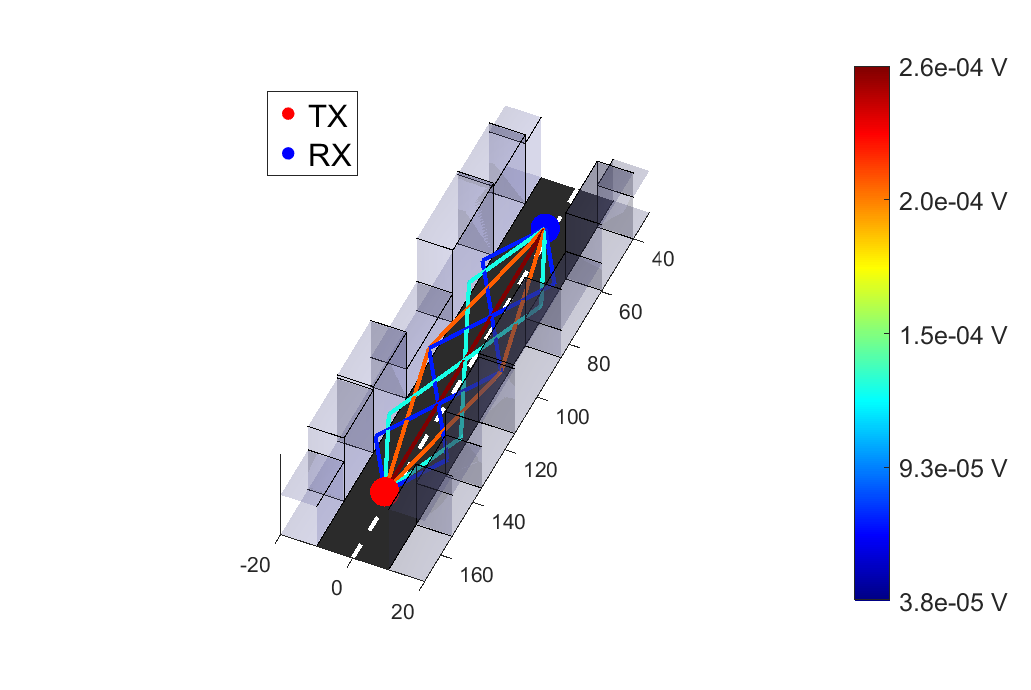
\includegraphics[width=0.8\textwidth]{3_2.eps}
    \caption{Received voltage for each ray}
    \label{fig:voltageDemo}
\end{figure}

\section{Power analysis}
\label{sec:power_analysis}

By varying the distance between the two communicating cars between 0 and 1000m, a comparison is made between the raytracing simulation and the theoretical model on figure \ref{fig:P_RX(d)}. The simulated power is computed by taking the square of $V_{OC}$ divided by $Z_L \mathbin{\|} Z_a$ (see figure \ref{fig:equivalent_electrical_circuit}) and the theoretical power is computed using equation \ref{eq:power_friis_simplified}.

\begin{figure}[H]
    \centering
    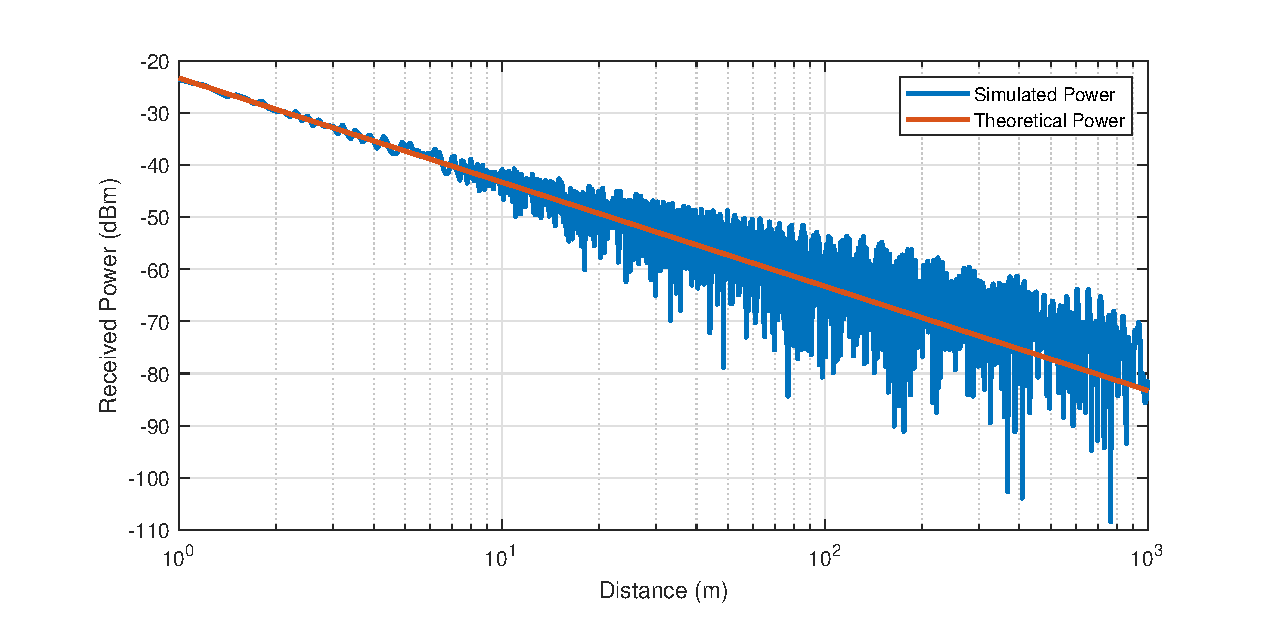
\includegraphics[width=1\textwidth]{3_3.eps}
    \caption{Received power as a function of the distance between the two cars}
    \label{fig:P_RX(d)}
\end{figure}

For short distances, the LOS ray is the only one contributing to the received power which explains the good match of the simulation with theory. \\
After a few meters, the multi path components (MPC) start to have an impact on the received power and the resulting interferences make the simulated power oscillate around the true power. \\
At greater distances and because of the limited number of bounces, one can clearly see the power is a multisine signal. This is because the reflection angles don't vary much with the distance at that point.\\

The oscillation around the expected power can be modeled with a Rice distribution as the LOS ray is the strongest one. The Rice factor $K$ is defined as the ratio between the power of the LOS ray and the power of the other rays:

\begin{align*}
    K = \frac{a_0^2}{\sum_{n=1}^{N}a_n^2}
\end{align*}

where $a_n$ is the amplitude of the $n^{th}$ ray with $a_0$ the amplitude of the LOS ray. As those amplitudes vary with distance, figure \ref{fig:K(d)} shows the rice factor as a function of the distance between the two cars. 

\begin{figure}[H]
    \centering
    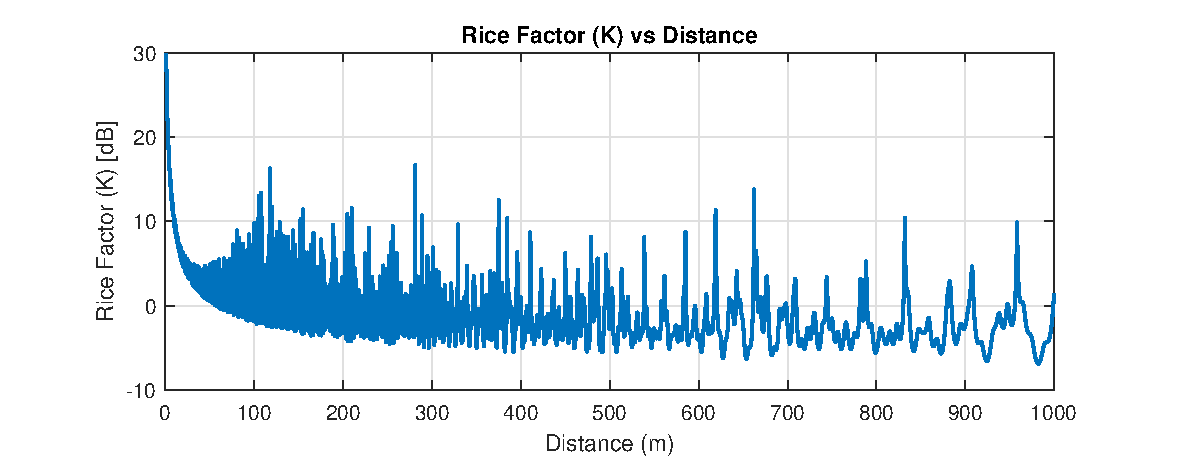
\includegraphics[width=1\textwidth]{3_4.eps}
    \caption{Rice factor as a function of the distance between the two cars. The highlighted point is the distance from which the LOS ray is not the strongest one anymore.}
    \label{fig:K(d)}
\end{figure}

The Rice factor is a good indicator of the portion of the power that is due to the LOS ray. The point at which it becomes smaller than 1 (or 0dB) is the point at which the power due to the LOS ray is equal to the sum of the power of the other rays. The Rice factor close to the emitter is high, which indicates that the fading is low. the Rice factor becomes smaller after only a few meters and, as seen in figure \ref{fig:P_RX(d)}, the received power oscillates around the expected value. This is the fading effect.\\

The average received power in local areas is computed using:

\begin{align*}
    <P_{\text{RX}}> &= \frac{1}{8 Z_a} \sum_{n=1}^{N} \left| V_{OC} \right|^2\\
    &= \frac{1}{45\pi} \sum_{n=1}^{N} \left| V_{\text{RX}} \right|^2\\
\end{align*}

Where the sum is done over all the received rays. Figure \ref{fig:average_power} shows the average received power in local areas with a width of 5m for an emitter placed at the intersection of the two roads. The power is in dBm as it quicly becomes very small. \\
Another simulation has been done with 2m wide local areas and an emitter placed a bit further from the intersection. The result is shown in figure \ref{fig:average_power_2m} and it can be clearly seen that it is really difficult to get any power when no LOS ray is present. \\
It must be mentioned that the simulation does not take any transmission ray into account. This is under the hypothesis that the walls of the buildings are thick enough to not let any ray pass through.

\begin{figure}[H]
    \centering
    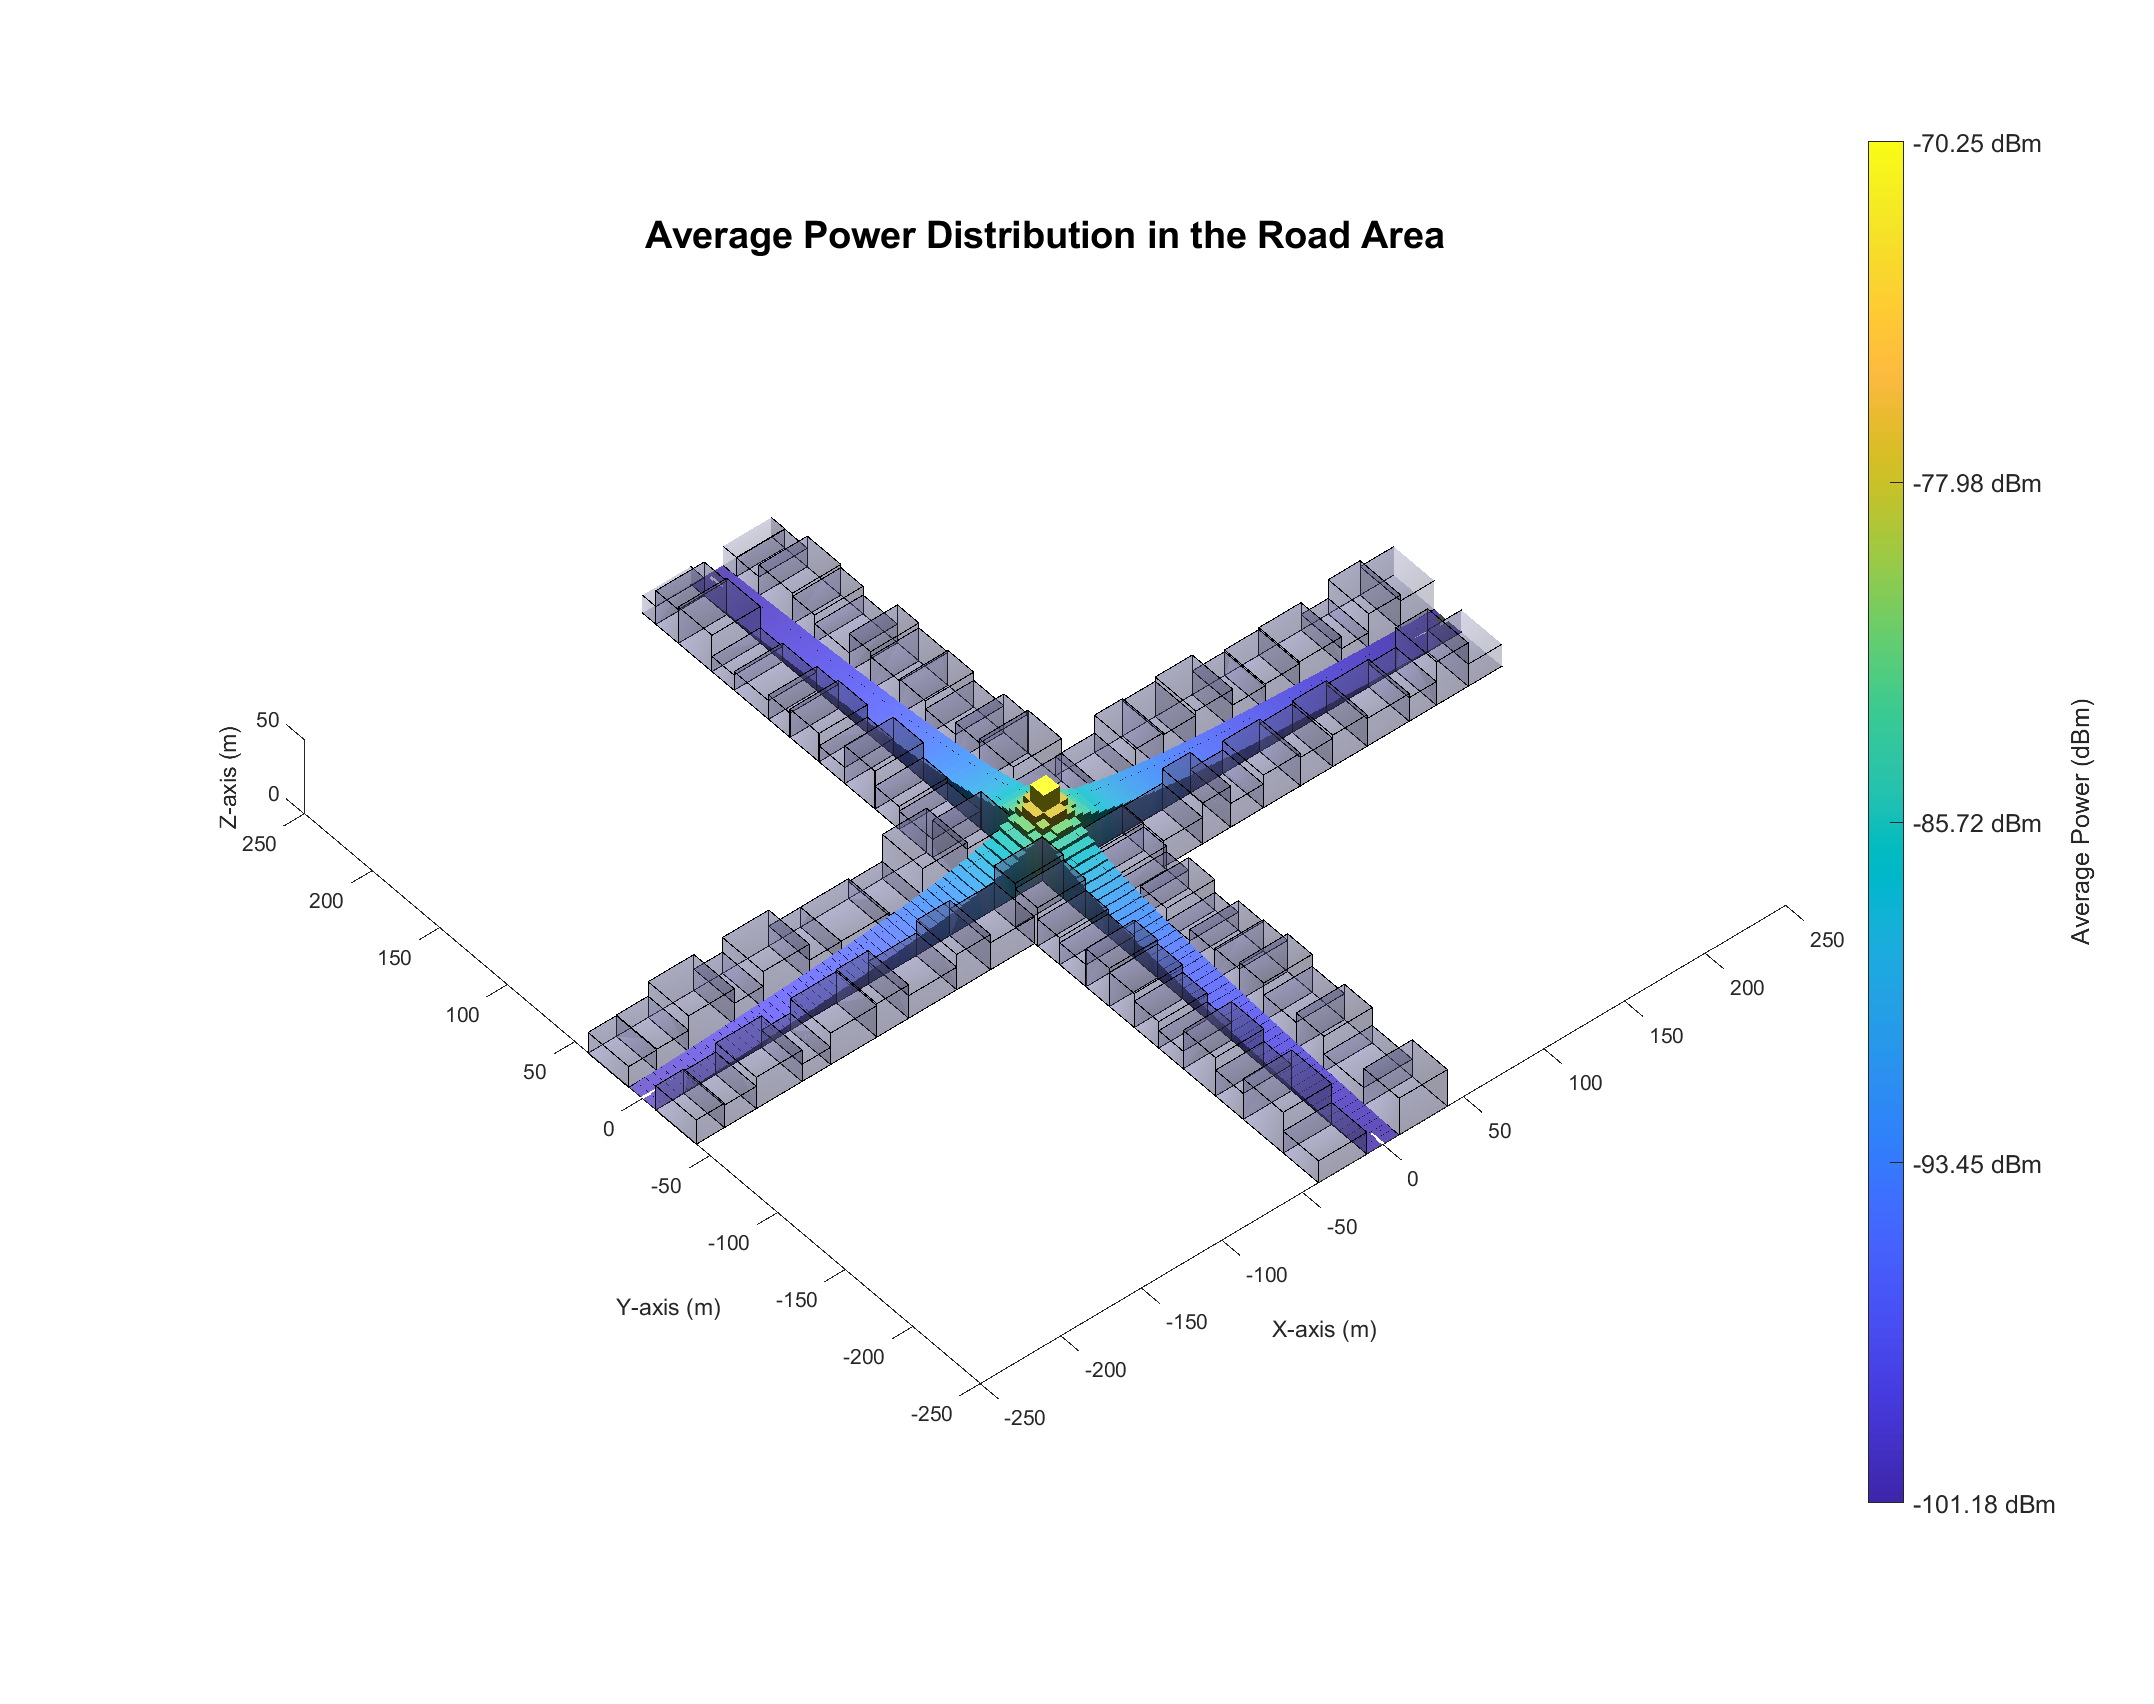
\includegraphics[width=1\textwidth]{3_5.eps}
    \caption{Average received power in local areas of 5m}
    \label{fig:average_power}
\end{figure}

\begin{figure}[H]
    \centering
    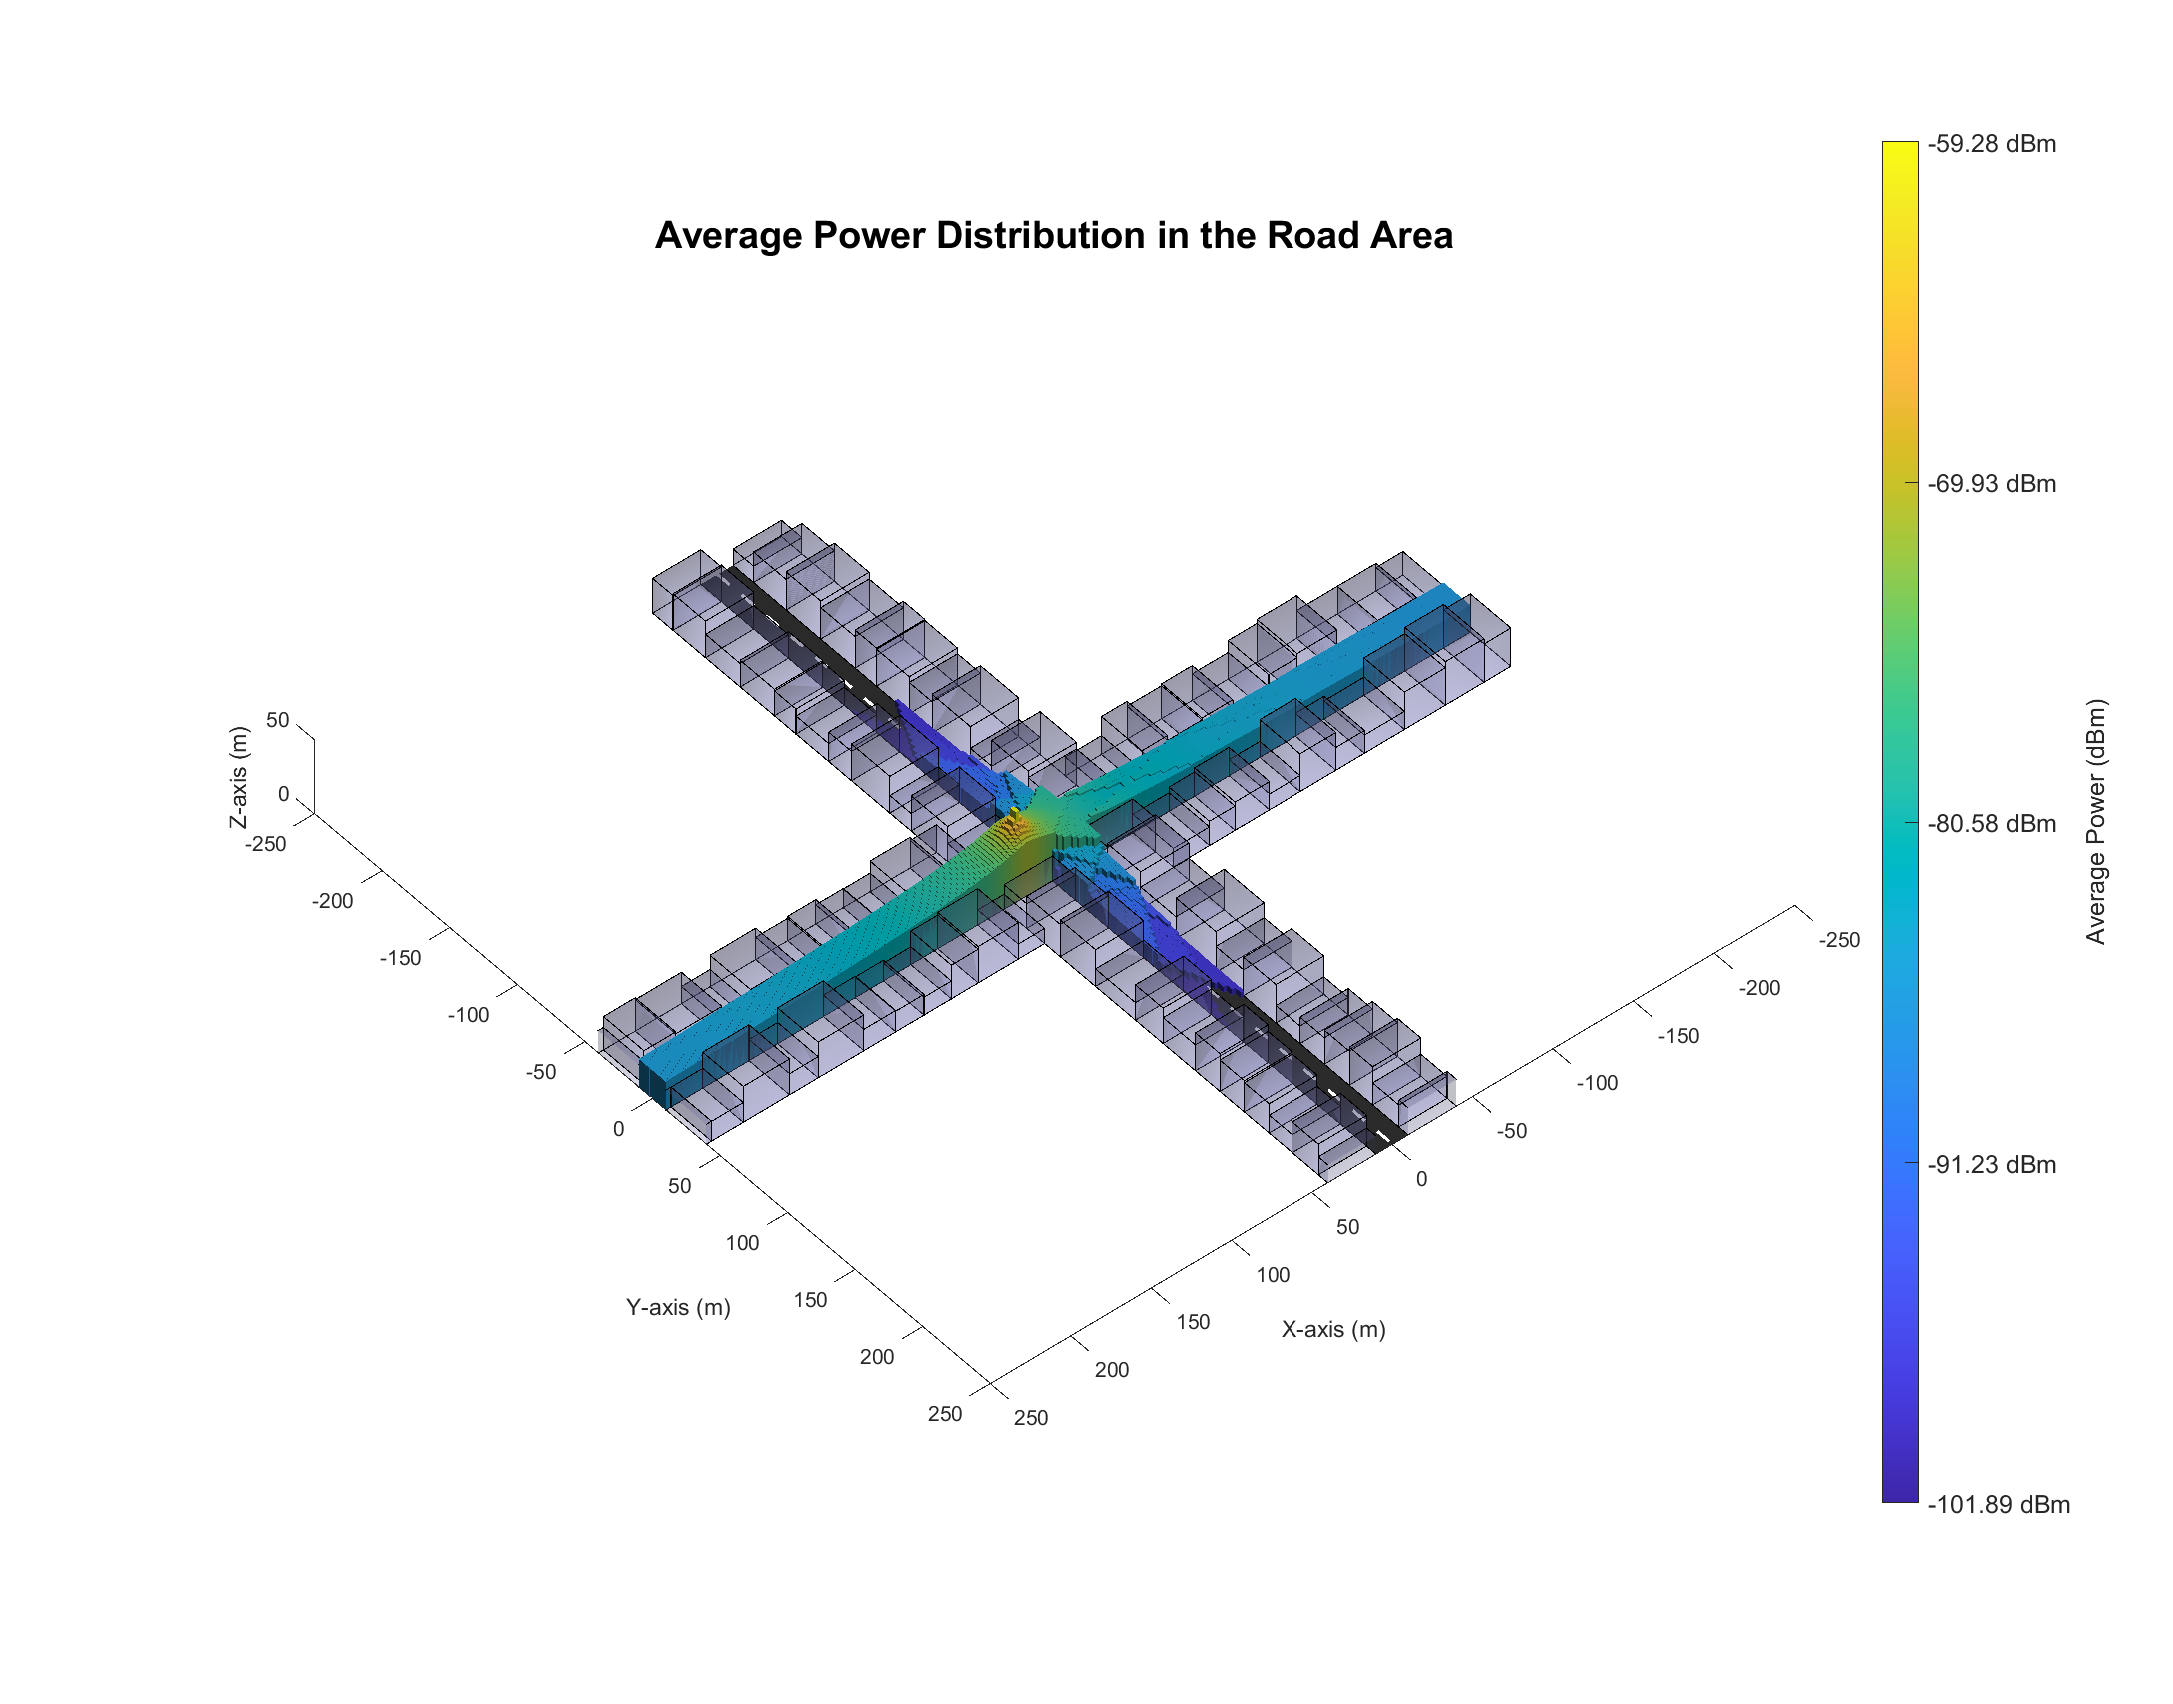
\includegraphics[width=1\textwidth]{3_5_alt.eps}
    \caption{Average received power in local areas of 2m}
    \label{fig:average_power_2m}
\end{figure}

\section{Full channel, narrowband model}

The pass loss of the channel $L(d)$ and the pass loss that does not depend on the antennas $L_0(d)$ are defined (with every term in dB) as:


\begin{subequations}
    \label{eq:pass_loss}
    \begin{align}
        L(d) &= P_{\text{TX}} - P_{\text{RX}}\\
        L_0(d) &= L(d) + G_{\text{TX}} + G_{\text{RX}}
    \end{align}
\end{subequations}

The canonical model for $L_0(d)$ is:

\begin{align*}
    L_0(d) = L_0(d_0) + 10 n log_{10} \left(\frac{d}{d_0}\right)
\end{align*}

In which the parameters $L_0$ and $n$ must be found to fit the values of the simulation. $d_0$ has been arbitrarily set to 1m. The result is shown in figure \ref{fig:pass_loss} and the resulting parameters give as path loss model:

\begin{align}
    \label{eq:pass_loss_model}
    L_0(d) = 58.501 + 15.6 \cdot log_{10} \left(\frac{d}{1\text{m}}\right)
\end{align}

\begin{figure}[H]
    \centering
    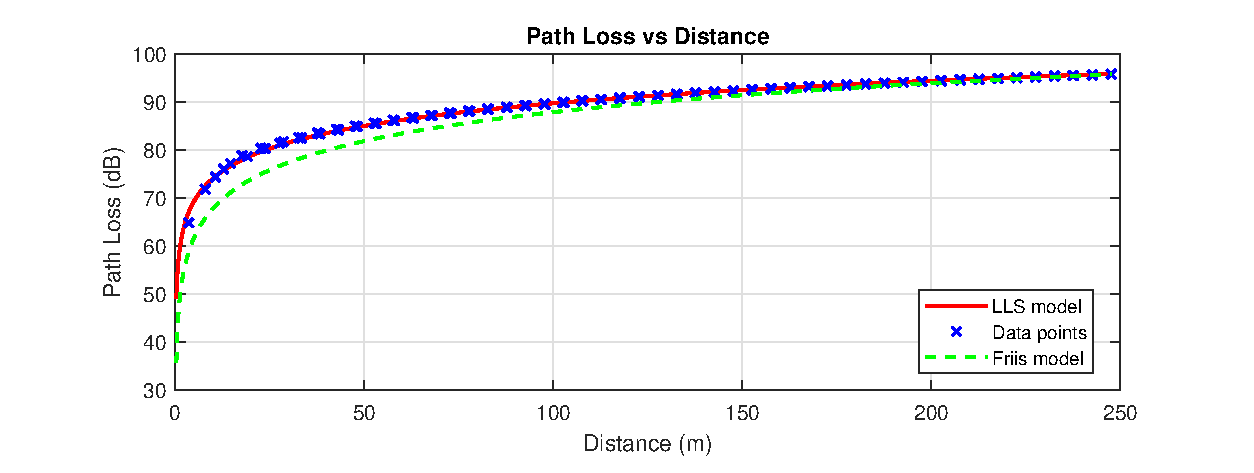
\includegraphics[width=1\textwidth]{3_5_model.eps}
    \caption{Pass loss of the channel and fitted model}
    \label{fig:pass_loss}
\end{figure}

As the LLS estimator only gives a "\textit{best fit}" to the data, there is still a parameter to define: the variability $\sigma_L$. It is the standard deviation of the path loss around the fitted model and its value here is:

\begin{equation*}
    \sigma_L = 0.30236 \quad \text{dB}
\end{equation*}

Regarding the communication reliability, it can be found under the assumption that the power variations due to shadowing is log-normal distributed. In this case, the probability of a successful communication is given by:

\begin{equation}
    \label{eq:pass_loss_probability}
    P_{\text{success}} = \frac{1}{2} \text{erfc}\left(\frac{M}{\sigma_L\sqrt{2}}\right) 
\end{equation}

Where $M$ is the fade margin, defined as the difference between the received power and the minimum power needed to decode the signal. The fade margins required for a certain communication reliability are given in table \ref{tab:fade_margins}. They have been found by plotting the error probability as a function of the fade margin (see figure \ref{fig:fade_margin}). \\
The cell range can also be computed for each value of $P_{\text{success}}$ using equation \ref{eq:pass_loss} and \ref{eq:pass_loss_model}. 

\begin{align*}
    L(d) &= P_{\text{TX}} - P_{\text{RX}}\\
    L_0(d_\text{max}) &= P_{\text{TX}} - P_{RX, \text{min}} + G_{\text{TX}} + G_{\text{RX}}\\
    58.501 + 15.6 \cdot log_{10} \left(\frac{d_{\text{max}}}{1\text{m}}\right) &= P_{\text{TX}} - P_{RX, \text{min}} + G_{\text{TX}} + G_{\text{RX}}
\end{align*}

The minimal received power $P_{RX, \text{min}}$ is the receiver sensitivity to which the fade margin is added. Putting the values of the left parameters in the equation gives:

\begin{align*}
    58.501 + 15.6 \cdot log_{10} \left(\frac{d_{\text{max}}}{1\text{m}}\right) &= 20 - (-70 + M) + 2 \times 10 \log_{10} \left(\frac{16}{3\pi}\right)\\
    \log_{10} \left(\frac{d_{\text{max}}}{1\text{m}}\right) &= \frac{36.1 - M}{15.6}\\
    d_{\text{max}} &= 10^{\frac{36.1 - M}{15.6}} \left[\text{m}\right]
\end{align*}

\begin{table}[H]
    \centering
    \begin{tabular}{|c|c|c|}
        \hline
        Communication reliability & Fade margin (dB) & Cell radius (m) \\ \hline
        50\% & 0 & 205.98 \\ \hline
        95\% & 0.497 & 191.41 \\ \hline
        99\% & 0.703 & 185.68 \\ \hline
    \end{tabular}
    \caption{Fade margins and cell radius for different communication reliability}
    \label{tab:fade_margins}
\end{table}

\begin{figure}[H]
    \centering
    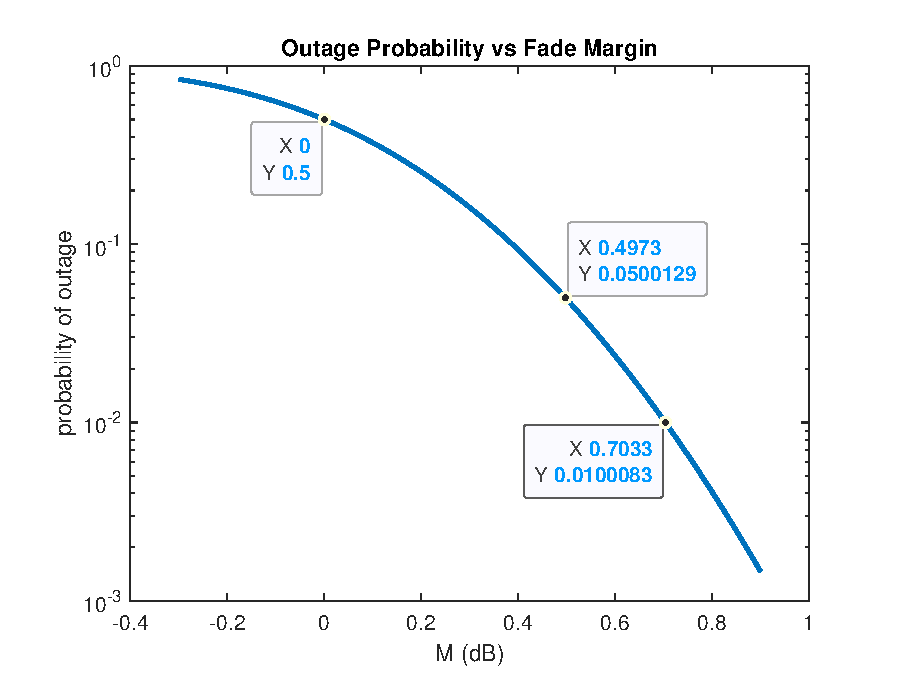
\includegraphics[width=1\textwidth]{3_7.eps}
    \caption{Fade margin as a function of the communication reliability, plotted using equation \ref{eq:pass_loss_probability}}
    \label{fig:fade_margin}
\end{figure}

\section{LOS channel, wideband model}
\label{sec:LOS_channel_wideband}

For the wideband model and if there is only a single ray, the impulse response of the channel is given by:

\begin{equation*}
    h(t) = \frac{e^{-j \frac{2\pi f_cd_1}{c}}}{d_1} \delta(t - \tau_1)
\end{equation*}

The impulse response and the corresponding transfer function (computed by taking the DFT of $h(t)$) are shown in figure \ref{fig:impulse_response} and \ref{fig:transfer_function}. 

\begin{figure}[H]
    \centering
    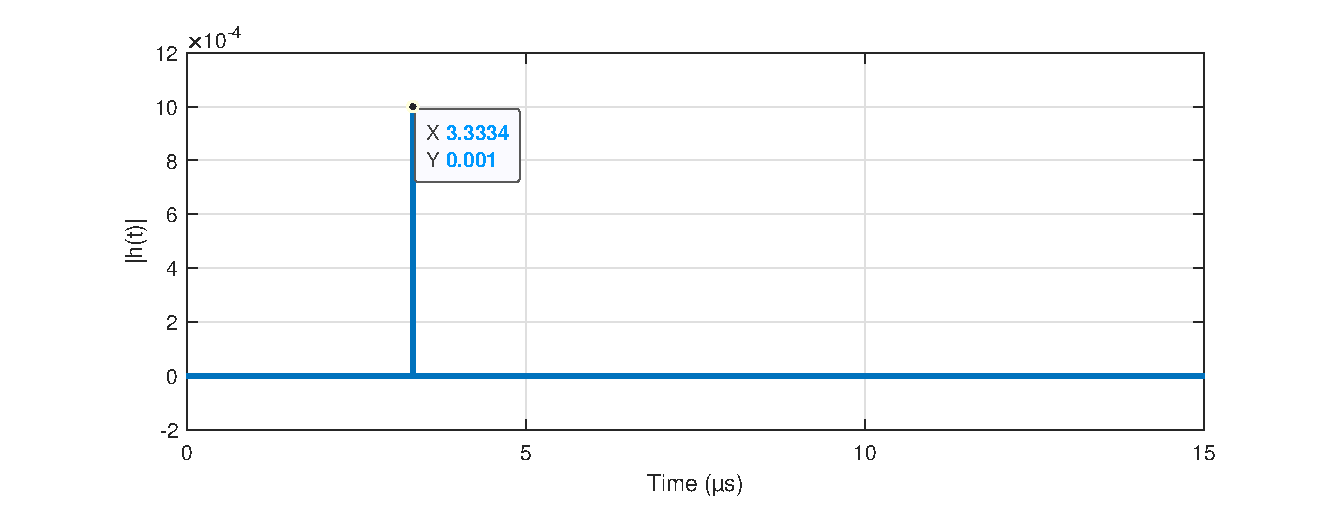
\includegraphics[width=1\textwidth]{4_1_temp.eps}
    \caption{Impulse response of the wideband channel with the LOS ray only} 
    \label{fig:impulse_response}
\end{figure}

\begin{figure}[H]
    \centering
    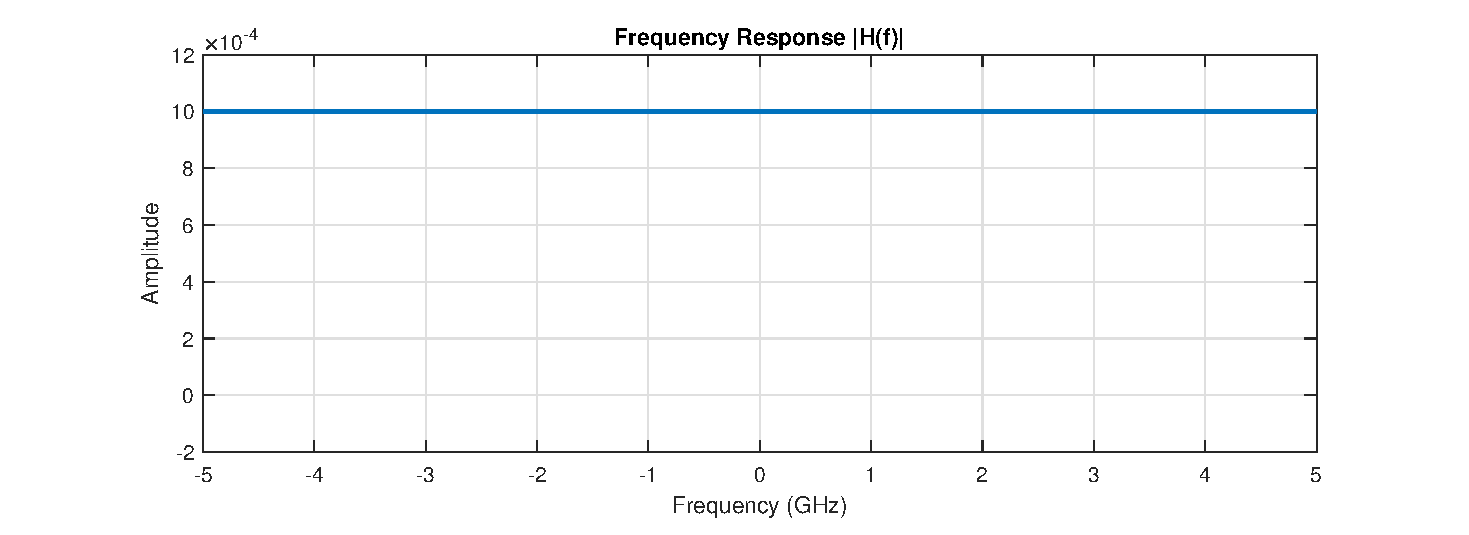
\includegraphics[width=1\textwidth]{4_1_freq.eps}
    \caption{Transfer function of the wideband channel with the LOS ray only}
    \label{fig:transfer_function}
\end{figure}

The impulse response is a single peak at a time corresponding to the time of flight of the LOS ray. The transfer function has a constant value over the frequency spectrum. This means that there is no frequency selectivity for a single ray, a result easily understandable as no frequency is less attenuated than another in free space. This is of course valid only because some assumptions have been made: there is no multipath propagation and no parasitic effects (gaseous absorption, rain attenuation, tropospheric scintillation, etc.).\\
Because of the limitted bandwidth of the channel, the tapped delay line model is used to compute $h_{\text{TDL}}(t)$. The previous impulse response did not take into the fact that the receiver is only able to sample at the time resolution of the system $\Delta\tau = \frac{1}{B}$, where B is its bandwidth. The TDL model is found by:

\begin{equation}
    h_{\text{TDL}}(t) = \sum_{l=0}^{L} h_l(t) \delta(t - l\Delta\tau)
    \label{eq:h_TDL}
\end{equation}
\begin{equation*}
    \text{where} \qquad h_l(t) = \sum_{n=1}^{N} \alpha_n(t) \text{sinc}\left(B(\tau_n - l\Delta\tau)\right)
\end{equation*}

In those equations, $L$ is the maximal index of the temporal taps (linked with the maximal allowed delay) and $N$ is the number of rays, which is simply $1$ in this case. $\alpha_1$ is different from the one defined in section \ref{sec:LOS_channel}, as it here takes the spacial dispersion into account:

\begin{equation*}
    \alpha_n = \prod_{b=1}^{B} \Gamma_{\perp, b} \cdot \frac{e^{\frac{-j2\pi f_c d_n}{c}}}{d_n} \qquad \text{where } B \text{ is the number of bounces of the } n^{th} \text{ ray}
\end{equation*}

When all of it is put together in equation \ref{eq:h_TDL}, the impulse response of the channel becomes:

\begin{equation*}
    h_{\text{TDL}}(t) = \sum_{l=0}^{L}\frac{e^{\frac{-j2\pi f_c d_1}{c}}}{d_1} \text{sinc}\left(B(\tau_1 - l\Delta\tau)\right) \delta(t - l\Delta\tau)
\end{equation*}

On figure \ref{fig:h_TDL_LOS}, the effect of the sinc function is clearly visible: the impulse response is no longer a single peak but the adjacent time bins (of size $\Delta\tau$) are now different from zero. This is because the receiver is not able to sample the signal at the exact time of flight of the ray. \\

\vspace{0.5cm}
\Large \textbf{More explanations needed}
\normalsize\\

\begin{figure}[H]
    \centering
    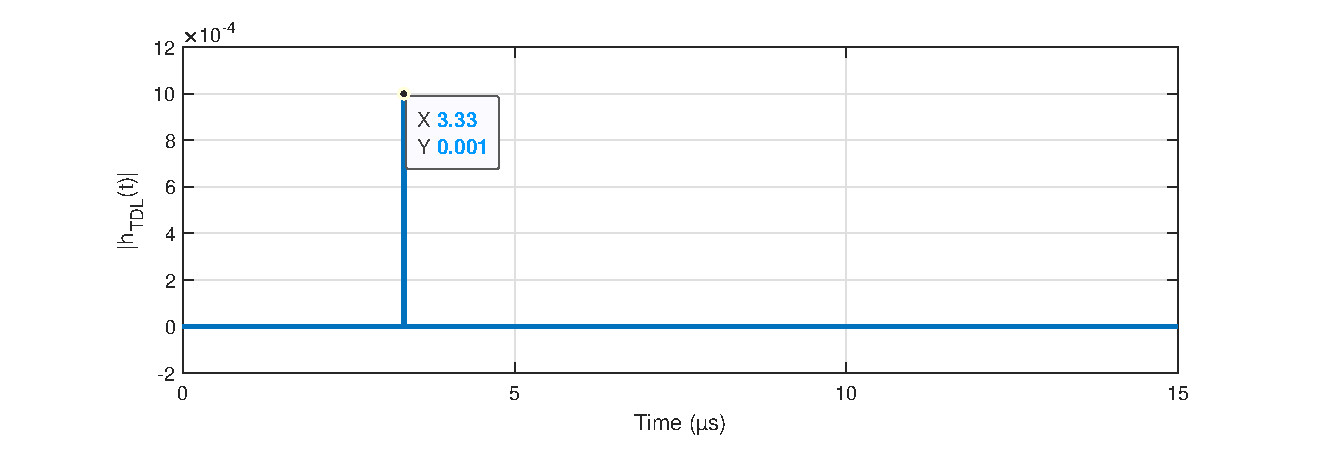
\includegraphics[width=1\textwidth]{4_2.eps}
    \caption{TDL impulse response of the wideband channel with the LOS ray only}
    \label{fig:h_TDL_LOS}
\end{figure}

\section{Full channel, wideband model}

This section will do the same analysis as the previous one but for multiple rays. The impulse response and the corresponding transfer function are shown in figure \ref{fig:impulse_response_full} and \ref{fig:transfer_function_full}. \\
The impulse response plot is zoomed in so the different peaks are visible. Because of those peaks, some frequencies are more attenuated than others during their propagation through the channel. This is the reason why the transfer function is not constant anymore. \\
The transfer function plot is also only partially shown in order to focus around the carrier frequency $f_c = 5.9$GHz. This analysis shows that this choice for $f_c$ is not optimal as the amplitude of $H(f)$ is low around this frequency. A wiser choice would have been to choose a frequency around $f_c = 6.5$GHz. Even though the transfer function is not maximal there, it does not vary much around it whereas a change of only $10$ MHz above $5.9$GHz could diminish the amplitude of the transfer function by half.

\begin{figure}[H]
    \centering
    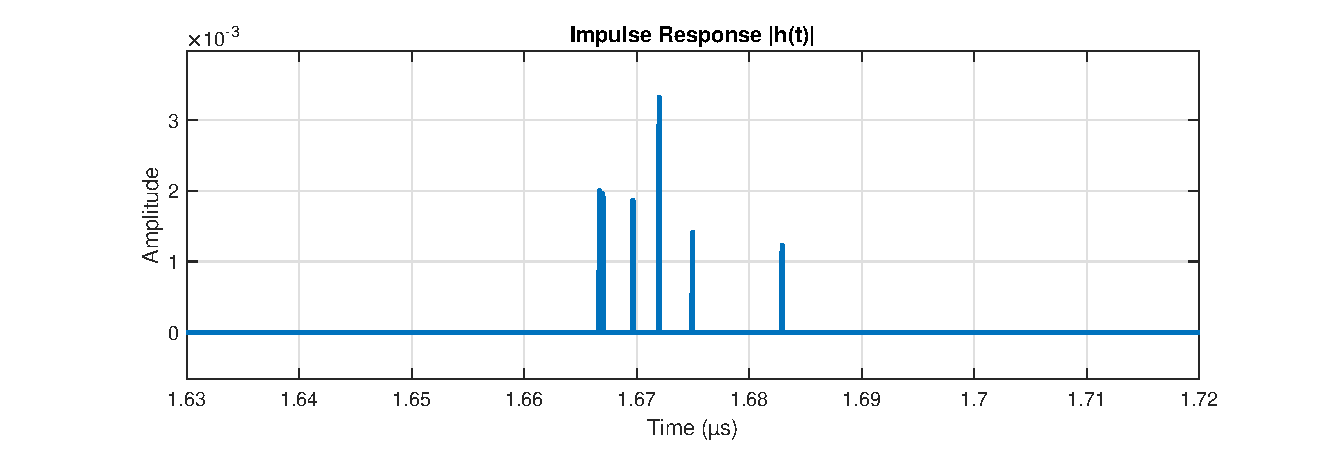
\includegraphics[width=1\textwidth]{5_1.eps}
    \caption{Impulse response of the wideband channel with multiple rays}
    \label{fig:impulse_response_full}
\end{figure}

\begin{figure}[H]
    \centering
    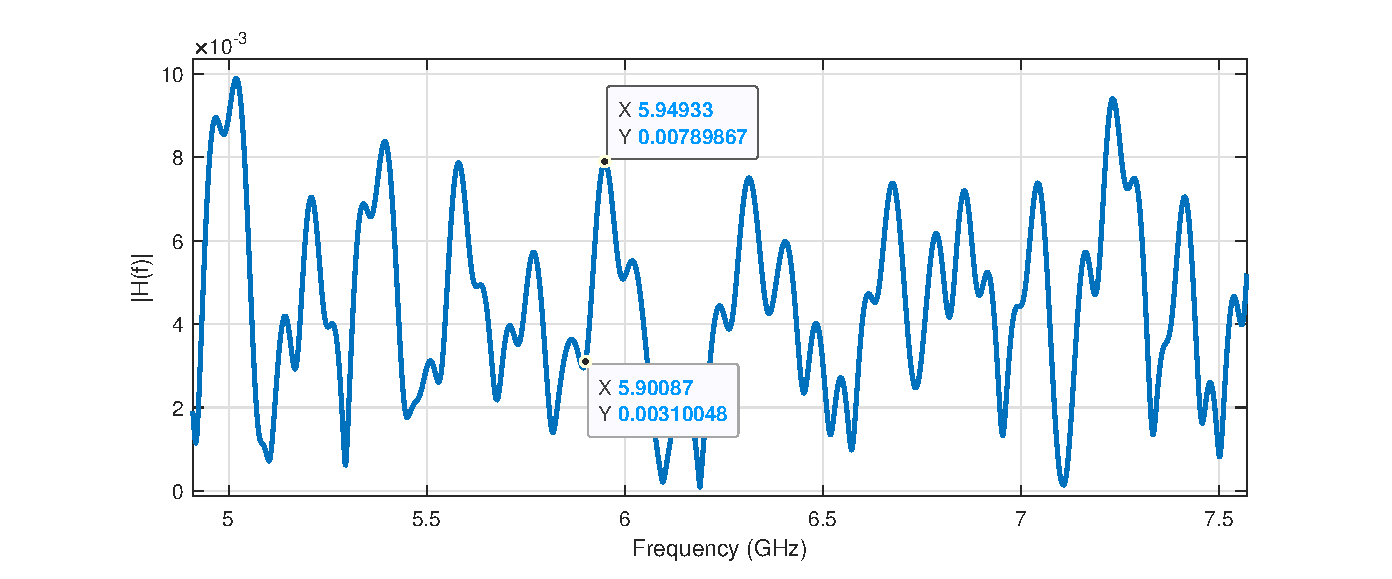
\includegraphics[width=1\textwidth]{5_2.eps}
    \caption{Transfer function of the wideband channel with multiple rays}
    \label{fig:transfer_function_full}
\end{figure}

The impulse response of the tapped delay line model is computed using the same method as in section \ref{sec:LOS_channel_wideband} and it is plotted together with the one in with the LOS ray only on figure \ref{fig:impulse_response_TDL}. 

\begin{figure}[H]
    \centering
    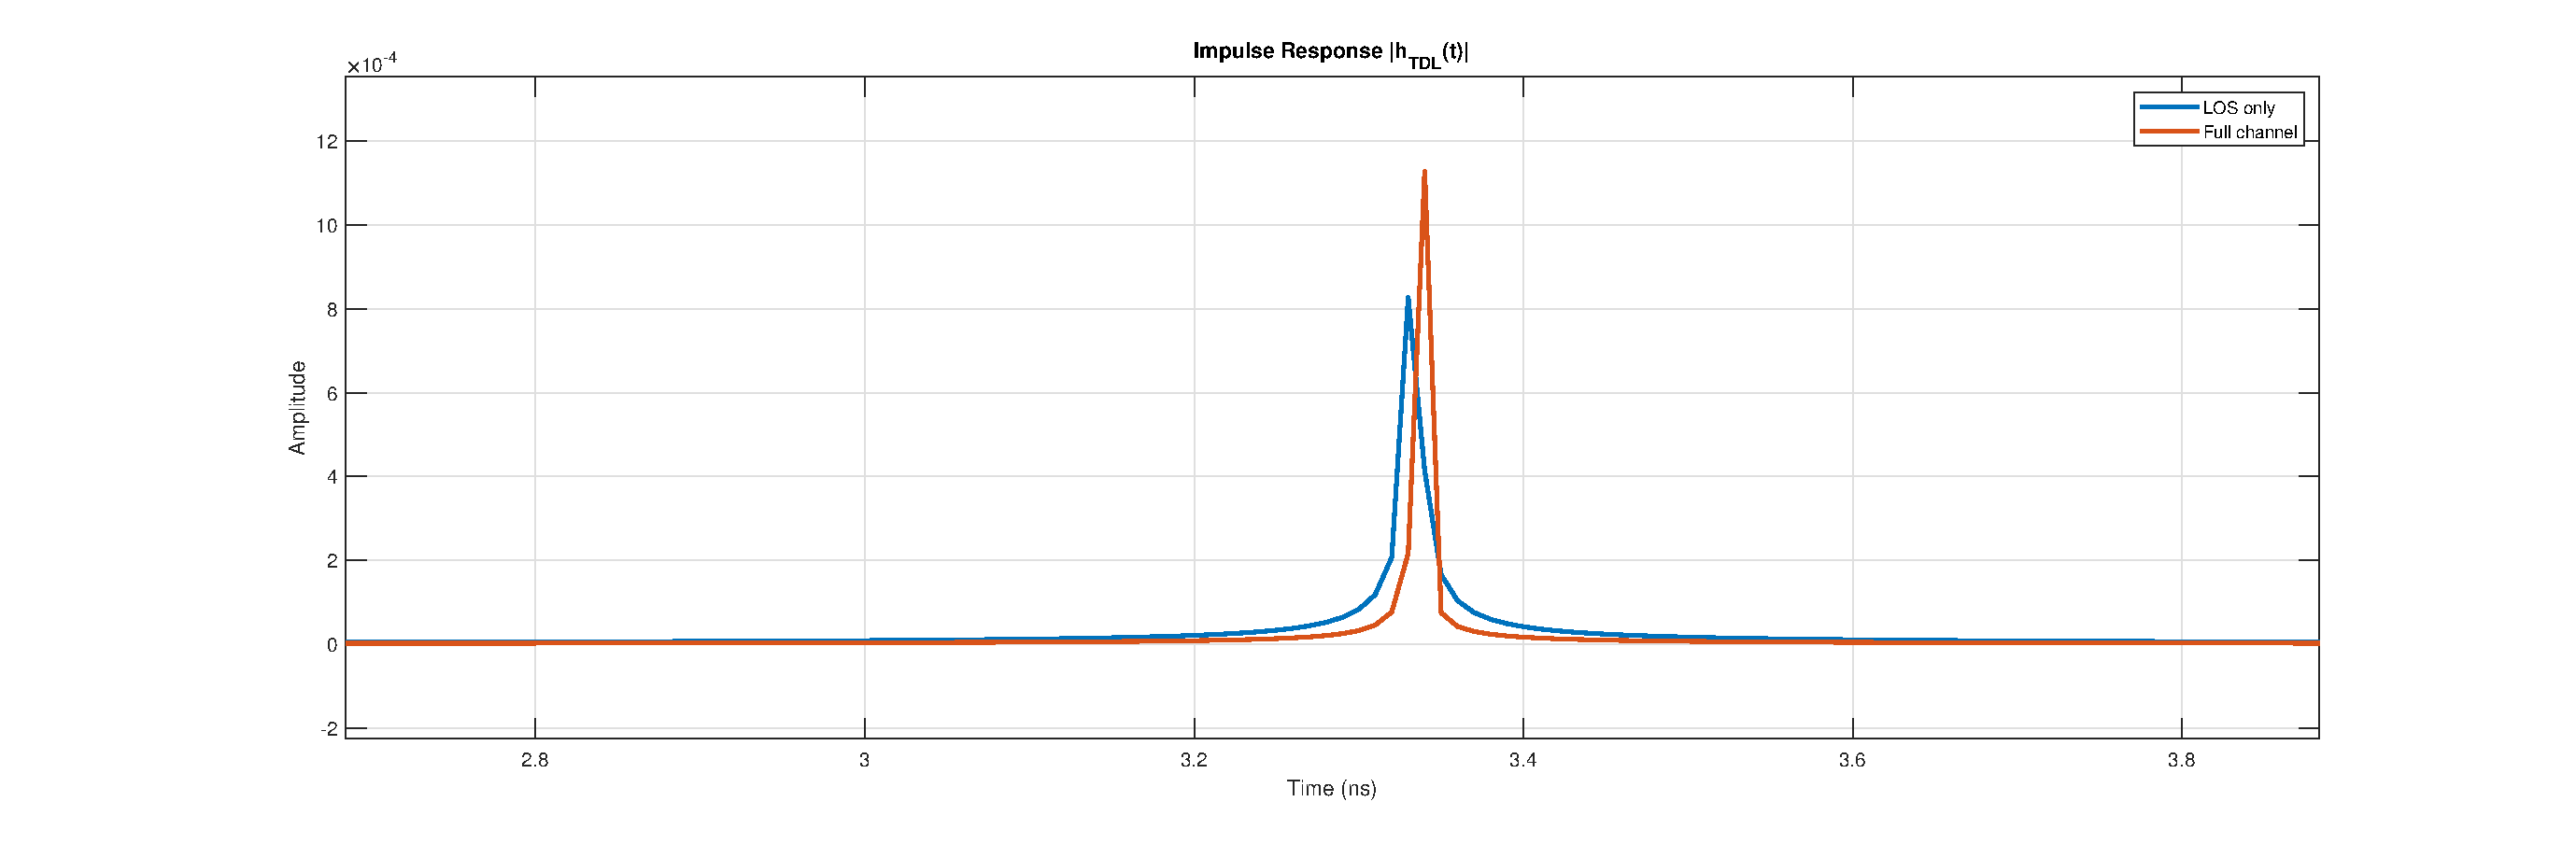
\includegraphics[width=1\textwidth]{comparison_h_TDL.eps}
    \caption{Comparison of $h_{\text{TDL}}$ for the LOS ray only and the full channel}
    \label{fig:impulse_response_TDL}
\end{figure}

Taking the MPC into account makes $h_{\text{TDL}}$ reach a higher value than the one with the LOS ray only. Because the bandwidth of the channel is lower than the coherence bandwidth (defined as the inverse of the delay between the first and last incoming ray), all the rays are arriving approximately at the same time. \\
To verify this, the same script has been used with 15 bounces instead of 3. The coherence bandwidth decreased from $123$MHz to as low as $6$MHz. The impulse response is shown on figure \ref{fig:impulse_response_TDL_15_bounces} and separate peaks are now visible.

\begin{figure}[H]
    \centering
    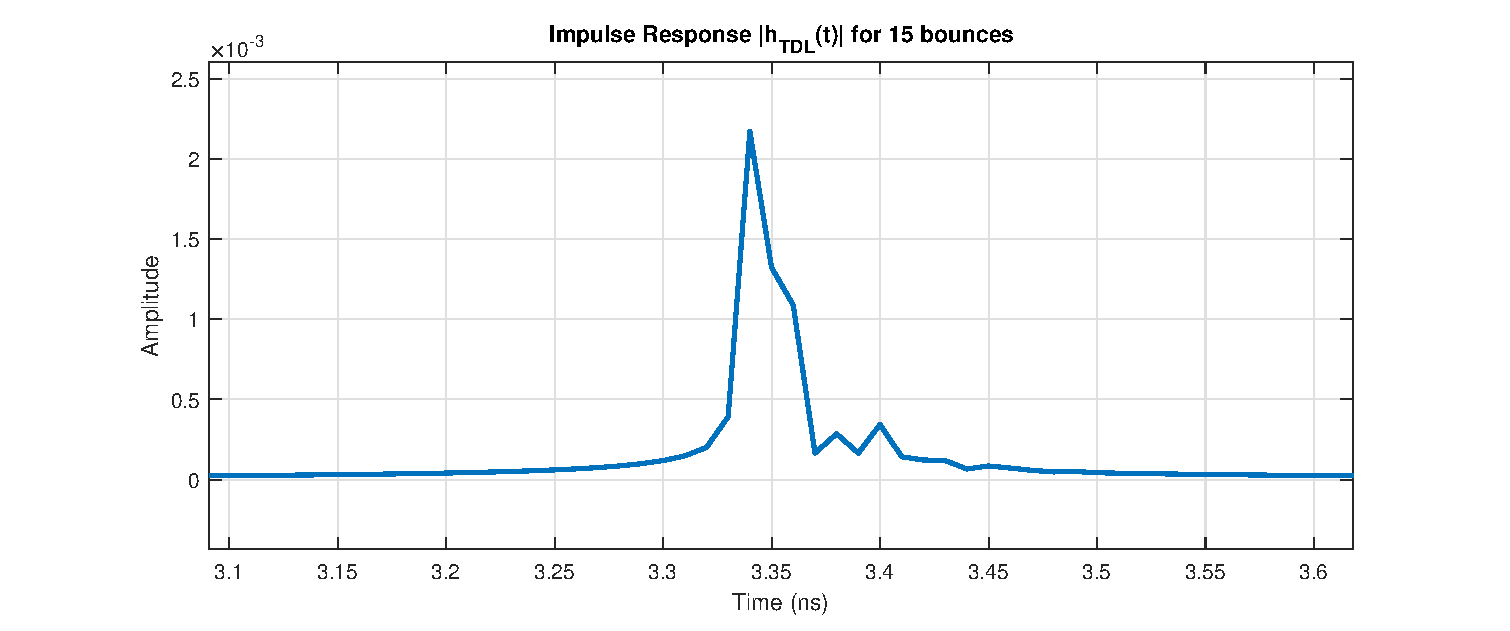
\includegraphics[width=1\textwidth]{5_3_15_bounces.eps}
    \caption{Impulse response of the wideband channel with multiple rays and 15 bounces}
    \label{fig:impulse_response_TDL_15_bounces}
\end{figure}



\chapter{Further analysis}
\section{Description}
As shown on 3D figures, the simulated road contains a $90^\circ$ crossing. This section will analyze what happens in the case of cars from different roads communicating with each other. The rays that would pass through buildings are supposed to be absorbed and are therefore not taken into account. Because of this, a lot of rays are removed and there is a need for a higher number of bounces. \\
\section{Power analysis}
The power analysis is done the same way as in section \ref{sec:power_analysis} but with a different setup. The 3D plot \ref{fig:3D_2} shows the averaged power received in local areas of 5m. with the transmitting car placed at 25m from the intersection center.

\begin{figure}
    \centering
    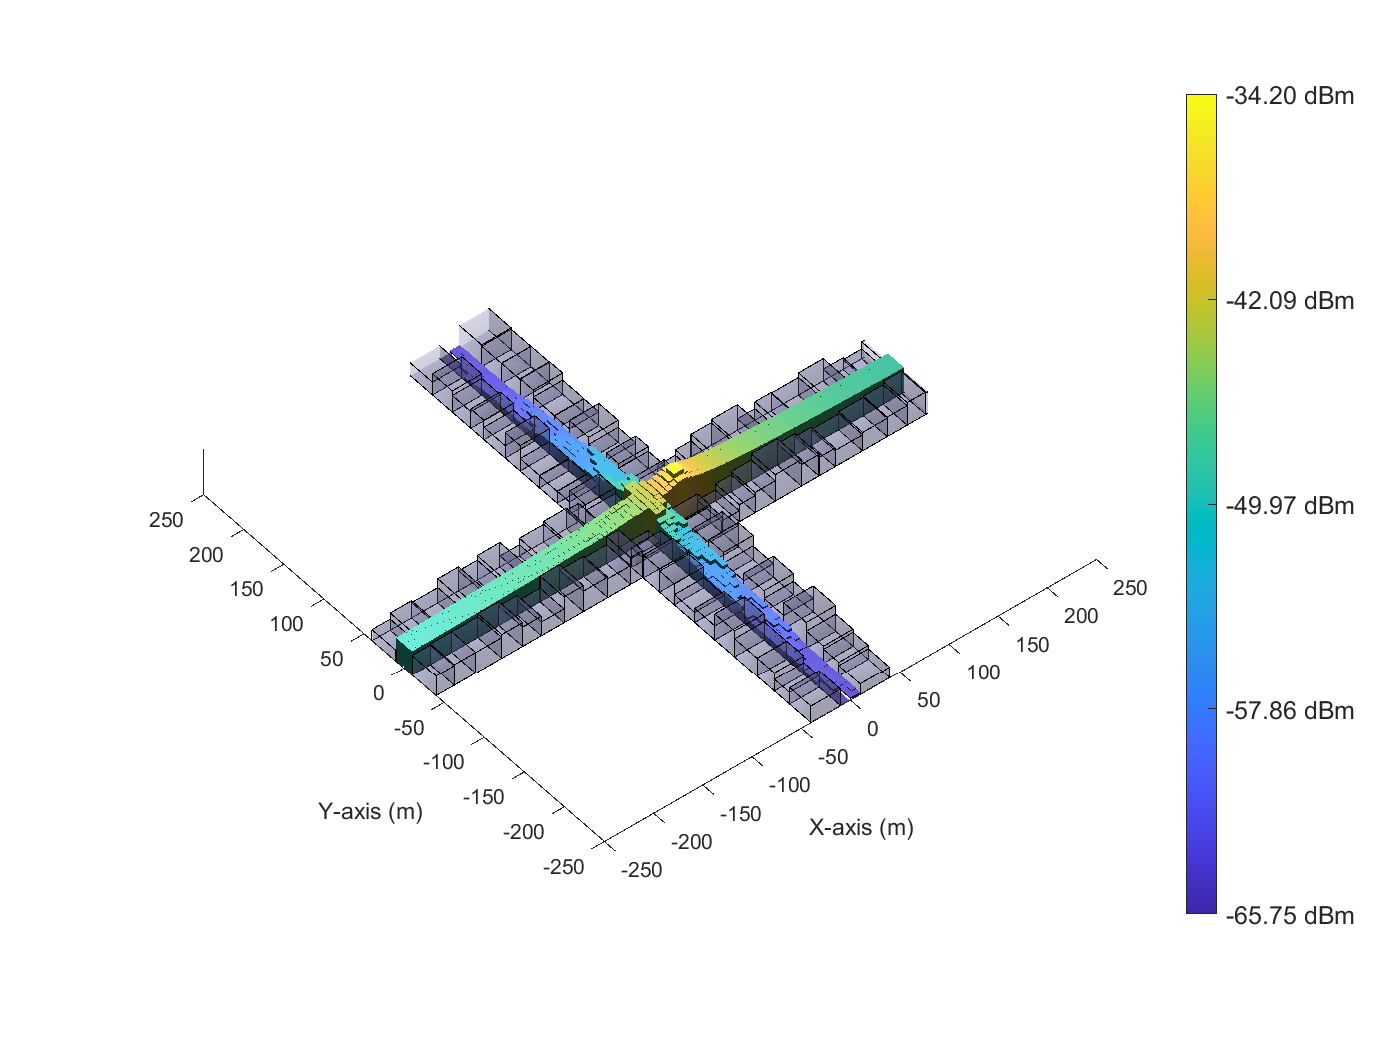
\includegraphics[width=1\textwidth]{6_1.eps}
    \caption{Average received power in local areas of 5m for a car placed at 25m from the intersection center with a maximal number of bounces of 6}
    \label{fig:3D_2}
\end{figure}

As one can see, the power is now much less homogeneous than in the previous case and it becomes even more obvious when trying to model it. This was done the same way as previously and it is shown in figure \ref{fig:pass_loss_2}. The fitted model is:

\begin{align*}
    L_0(d) &= 45.561 + 28.147 \cdot log_{10} \left(\frac{d}{1\text{m}}\right)\\
    \text{with } \sigma_L &= 12.7679 \quad \text{dB}
\end{align*}

\huge Redo with only the perpendicular points maybe?\\
\normalsize 

The data points in figure \ref{fig:pass_loss_2} can be split in two groups: the points with a lower path loss, that stay close to the Friis model, and the points with a higher path loss. The first group corresponds to the positions on the same road as the transmitter and the values are quiet close to the ones in figure \ref{fig:pass_loss}. \\
The second group corresponds to the cars on the perpendicular road. Those have a much higher pass loss as a lot of rays are absorbed by the buildings. The fitted model being minimizing the least square error for the whole dataset, it is unable to properly fit to the data points. This is easily measured by the standard deviation which is, in this case, 40 times higher than the one computed previously. \\

\begin{figure}
    \centering
    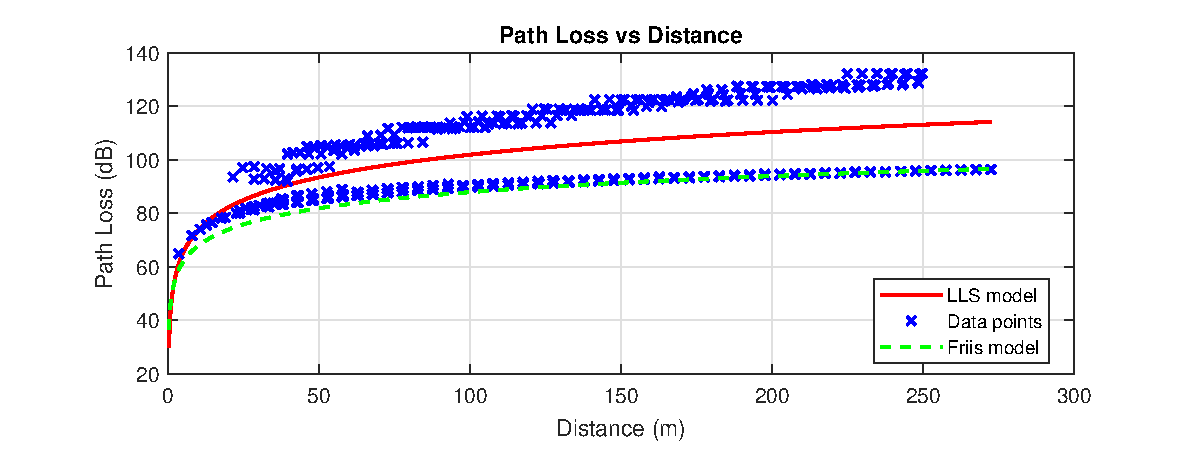
\includegraphics[width=1\textwidth]{6_2.eps}
    \caption{Pass loss of the channel and fitted model for a car placed at 25m from the intersection center with a maximal number of bounces of 6}
    \label{fig:pass_loss_2}
\end{figure}

\section{Communication reliability}

The change in the model implies that the cell radius must be recomputed. A table with the fade margins and the cell radius is shown below. Because the variability is much higher, the range of the cell radius is rapidly decreasing when the communication reliability becomes higher. \\

\begin{table}[H]
    \centering
    \begin{tabular}{|c|c|c|}
        \hline
        Communication reliability & Fade margin (dB) & Cell radius (m) \\ \hline
        50\% & 0 & 55.22 \\ \hline
        95\% & 20.979 & 9.92 \\ \hline
        99\% & 29.721 & 4.855 \\ \hline
    \end{tabular}
    \caption{Fade margins and cell radius for different communication reliability}
    \label{tab:fade_margins_2}
\end{table}

Note that in such a case, the cell radius is not a good indicator of the range of the car. One can indeed see that a 99\% communication reliability is only possible for a car placed at less than 5m from the emitter but at such distances, there is no wall between the two cars and the situation is identical to the one in section \ref{sec:power_analysis}. \\
A more realistic number is the one for 50\% communication reliability. At such distances, the intersection has indeed an effect on the transmission and comparing it with the 200m in the straight road scenario, it is clear that the intersection has a big impact on the communication. \\

%\printglossary

%\printglossary[type=\acronymtype]

%Bibliography
%\nocite{*}
%\printbibliography[type=article,title=Articles]

\end{document}	
